\exercise{7\textbar 1}{Wettbewerbspolitik}

\textbf{Aufgabe:}

\begin{enumerate}[label=(\alph*)]
    \item Welche Motive haben Unternehmen, wettbewerbsbeschränkende Maßnahmen zu verfolgen?
    \item Wie wahrscheinlich ist es, dass es zu Kartellabsprachen unter den Unternehmen kommt?
    \item Was unterscheidet eine horizontale von einer vertikalen Fusion?
    \item Was versteht man unter einer „marktbeherrschenden Stellung“?
    \item Unter welchen Voraussetzungen sind in Europa staatliche Subventionen an Unternehmen erlaubt, sodass diese nicht unter das Beihilfeverbot fallen?
\end{enumerate}

\solution{
\begin{enumerate}[label=(\alph*)]
    \item \textbf{Motive für wettbewerbsbeschränkende Maßnahmen:}
    \begin{itemize}
        \item Reduktion des Konkurrenzdrucks und Vermeidung von Unsicherheiten.
        \item Sicherung höherer Gewinne durch mehr Marktmacht und höhere Markteintrittsbarrieren.
        \item Realisierung von Kosteneinsparungen (Economies of Scale) und Synergieeffekten.
        \item Erreichen einer dominierenden Marktposition oder Abschreckung potenzieller Konkurrenten.
        \item Persönliche Vorteile der Unternehmensführung wie Einkommenssteigerungen oder Prestigegewinne.
    \end{itemize}

    \item \textbf{Wahrscheinlichkeit von Kartellabsprachen:}
    \begin{itemize}
        \item Höhere Wahrscheinlichkeit bei:
        \begin{itemize}
            \item Wenigen Anbietern auf dem Markt.
            \item Hohen Markteintrittsbarrieren.
            \item Homogenen Gütern.
            \item Unelastischer Nachfrage.
        \end{itemize}
        \item Kartelle dienen der Reduktion der Wettbewerbsintensität und langfristigen Planbarkeit (z. B. Mitarbeiter, Investitionen).
    \end{itemize}

    \item \textbf{Unterschied zwischen horizontaler und vertikaler Fusion:}
    \begin{itemize}
        \item \textbf{Horizontale Fusion:}
        \begin{itemize}
            \item Zusammenschluss von Unternehmen derselben Branche und Produktions- oder Handelsstufe.
        \end{itemize}
        \item \textbf{Vertikale Fusion:}
        \begin{itemize}
            \item Zusammenschluss von Unternehmen entlang vor- oder nachgelagerter Wertschöpfungsstufen.
            \item Übernahme von Zulieferern oder Abnehmern.
        \end{itemize}
    \end{itemize}

    \item \textbf{Definition einer marktbeherrschenden Stellung:}
    \begin{itemize}
        \item Ein Unternehmen ist marktbeherrschend, wenn es die Fähigkeit besitzt, Preise, Produktionsmengen oder Marktbedingungen ohne wirksamen Wettbewerb zu beeinflussen.
        \item Dies schließt die Beherrschung eines wesentlichen Teils des Marktes ein.
    \end{itemize}

    \item \textbf{Voraussetzungen für staatliche Subventionen in Europa:}
    \begin{itemize}
        \item Staatliche Beihilfen sind grundsätzlich nach Art. 107 Abs. 1 AEUV verboten, wenn sie den Wettbewerb im Binnenmarkt verfälschen oder zu verfälschen drohen.
        \item Ausnahmen sind möglich, wenn Subventionen:
        \begin{itemize}
            \item Zur Förderung benachteiligter Regionen dienen.
            \item Forschung und Entwicklung unterstützen.
            \item Den Umweltschutz verbessern.
            \item Kleine und mittlere Unternehmen fördern.
            \item Ausbildungsprogramme oder Arbeitsplätze für Arbeitslose schaffen.
        \end{itemize}
        \item Beispiel: Die EU-Kommission verpflichtete Irland, 13 Mrd. Euro an illegal gewährte Steuervergünstigungen von Apple zurückzufordern.
    \end{itemize}
\end{enumerate}
}
\exercise{7\textbar 2}{Marktversagen versus Staatsversagen}
\begin{itemize}
    \item \textbf{Fragestellung:} Was versteht man unter Staatsversagen und was könnten die Gründe dafür sein?
\end{itemize}

\solution{
\textbf{Marktversagen versus Staatsversagen}
\begin{itemize}
    \item Auch wenn Marktversagen vorliegt, ist dies keine hinreichende Bedingung für staatliche Eingriffe.
    \item Es besteht die Möglichkeit, dass der Staat bzw. die staatliche Politik versagt.
    \item Marktversagen muss gegenüber dem Staatsversagen abgewogen werden, bevor gehandelt wird.
    \item \textbf{Definition:}
        \begin{itemize}
            \item Staatsversagen liegt vor, wenn staatliche Eingriffe ins Marktgeschehen zu neuen Problemen führen oder selbst mit Mängeln behaftete Marktlösungen verursachen.
        \end{itemize}
    \item \textbf{Beispiele für Staatsversagen:}
        \begin{itemize}
            \item Geregelte Marktzugangsbeschränkungen und Verzerrungen des Wettbewerbs durch Subventionen für bestimmte Marktteilnehmer.
            \item Sozialwohnungen, bei denen marktwirtschaftlich bessere Lösungen ignoriert werden.
        \end{itemize}
    \item Ineffizienzen bzw. Wohlstandsverluste durch staatliche Aktivitäten haben unterschiedliche Ursachen.
    \item Häufig sind politische Entscheidungsträger nicht in der Lage, die Präferenzen der Bürger ausreichend zu ermitteln.
    \item \textbf{Weitere Gründe:}
        \begin{itemize}
            \item Staatliche Leistungen werden zu „unentgeltlich“ oder zu nicht kostendeckenden Preisen angeboten.
            \item Unvollständige Informationen der Politiker eröffnen Interessengruppen überproportionalen Einfluss.
            \item Politiker handeln oft im Sinne von Wiederwahlwahrscheinlichkeit, Macht und Prestige.
            \item Konjunkturelle Schwankungen können durch staatliches Verhalten verstärkt werden.
        \end{itemize}
\end{itemize}
}

\exercise{7\textbar 3}{Höchstpreise}
\begin{enumerate}[label=(\alph*)]
    \item Wozu dienen Höchstpreise?
    \item Was passiert, wenn ein Höchstpreis über dem Marktpreis festgelegt wird?
    \item Wer bestimmt die gehandelte Menge bei einem festgelegten Höchstpreis?
    \item Welche Konsequenzen ergeben sich bei einem Nachfrageüberhang bei Festlegung eines Höchstpreises?
    \item Warum kann sich die Situation auf dem offiziellen Markt bei Festlegung eines Höchstpreises noch verschärfen?
    \item Welche Maßnahmen kann der Staat ergreifen, um die negativen Folgen einer Höchstpreisregelung zu mildern bzw. zu verhindern?
\end{enumerate}

\solution{
\begin{enumerate}[label=(\alph*)]
    \item \textbf{Wozu dienen Höchstpreise?}\\
    Höchstpreise sollen die Nachfrager besserstellen als bei freier Marktpreisbildung. Sie werden deshalb vor allem für lebensnotwendige Güter (z. B. Brot oder Wohnungsmieten) seitens des Staates angeordnet.

    \item \textbf{Was passiert, wenn ein Höchstpreis über dem Marktpreis festgelegt wird?}\\
    In diesem Fall kommt der Marktpreis zur Anwendung. Damit Höchstpreise ihre gewünschte Wirkung entfalten, müssen die Höchstpreise unter dem Gleichgewichtspreis liegen.

    \item \textbf{Wer bestimmt die gehandelte Menge bei einem festgelegten Höchstpreis?}\\
    Die Anbieter des Gutes bestimmen über die von ihnen festgelegte Menge des Angebots.\\
    \textbf{Hintergrund:}
    \begin{itemize}
        \item Ein Höchstpreis, der unterhalb des Gleichgewichtspreises liegt, führt dazu, dass die nachgefragte Menge steigt, während die angebotene Menge sinkt.
        \item Der Grund liegt darin, dass bei einem niedrigeren maximalen Preis einige Unternehmen ihre Grenzkosten nicht mehr decken können und aus dem Markt austreten.
        \item Es kommt zu einem Nachfrageüberhang, sodass viele Nachfrager leer ausgehen, da sich im Marktgleichgewicht immer nur die kürzere Marktseite durchsetzt.
    \end{itemize}

    \item \textbf{Welche Konsequenzen ergeben sich bei einem Nachfrageüberhang bei Festlegung eines Höchstpreises?}\\
    Vorausgesetzt, der Staat belässt es allein bei der Festsetzung eines Höchstpreises, kommt es zu einer Reihe von negativen Wirkungen:
    \begin{itemize}
        \item Nur die Nachfrager, die am schnellsten auf dem Markt sind (Windhundverfahren), oder die geduldigsten in der Warteschlange werden bedient.
        \item Es bildet sich ein Schwarzmarkt heraus, auf dem sich der illegale Preis als Marktpreis einstellt.
    \end{itemize}

    \item \textbf{Warum kann sich die Situation auf dem offiziellen Markt bei Festlegung eines Höchstpreises noch verschärfen?}\\
    Ist der Schwarzmarkt einmal etabliert:
    \begin{itemize}
        \item Unternehmen halten mehr und mehr Güter vom offiziellen Markt zurück, um sie auf dem Schwarzmarkt zu höheren Preisen zu verkaufen.
        \item Nachfrager nutzen den offiziellen Markt nur, um Güter auf dem Schwarzmarkt gewinnbringend weiterzuverkaufen.
        \item Das Angebotsdefizit auf dem offiziellen Markt verschärft sich.
    \end{itemize}

    \item \textbf{Welche Maßnahmen kann der Staat ergreifen, um die negativen Folgen einer Höchstpreisregelung zu mildern bzw. zu verhindern?}\\
    \begin{itemize}
        \item Staatliche Maßnahmen können das Angebot ausweiten (z. B. Subventionen, Zollsenkungen, staatliche Unternehmen).
        \item Alternativ kann die Nachfrage reduziert werden (z. B. Subventionen für Substitutionsgüter).
    \end{itemize}
    \begin{figure}[H]
        \centering
        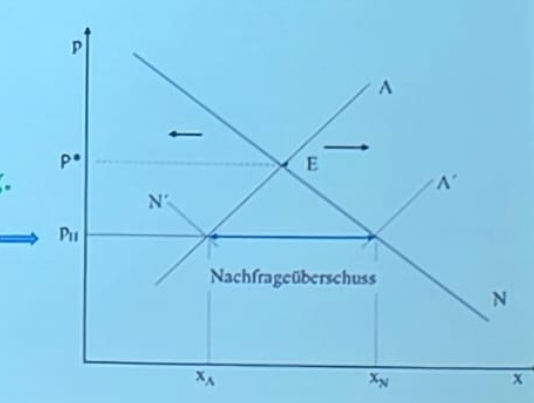
\includegraphics[width=0.4\textwidth]{figures/7_2.png}
        \caption{Marktmechanismen bei Höchstpreisen}
    \end{figure}
\end{enumerate}
}
\exercise{7\textbar 4}{Mindestpreise}
\begin{enumerate}[label=(\alph*)]
    \item Wozu dienen Mindestpreise?
    \item Muss ein Mindestpreis immer über dem Gleichgewichtspreis liegen?
\end{enumerate}

\solution{

\begin{enumerate}[label=(\alph*)]
    \item \textbf{Wozu dienen Mindestpreise?}
    \begin{itemize}
        \item Mit der Einführung von Mindestpreisen sollen die Anbieter besser gestellt werden.
        \item Die Festlegung von Mindestpreisen bedeutet, dass der Marktpreis für ein Gut eine bestimmte Höhe nicht unterschreiten, wohl aber überschreiten darf.
        \item Eingesetzt wird er hauptsächlich dort, wo den Anbietern ein bestimmtes Einkommen gesichert werden soll (z. B. in der Landwirtschaft).
    \end{itemize}

    \item \textbf{Muss ein Mindestpreis immer über dem Gleichgewichtspreis liegen?}
    \begin{itemize}
        \item Ja, der Mindestpreis muss über dem Gleichgewichtspreis liegen.
        \item Ihn darunter festzulegen, bliebe ohne praktische Auswirkung, da dann der höher liegende Marktpreis verwirklicht würde.
    \end{itemize}
\end{enumerate}
}

